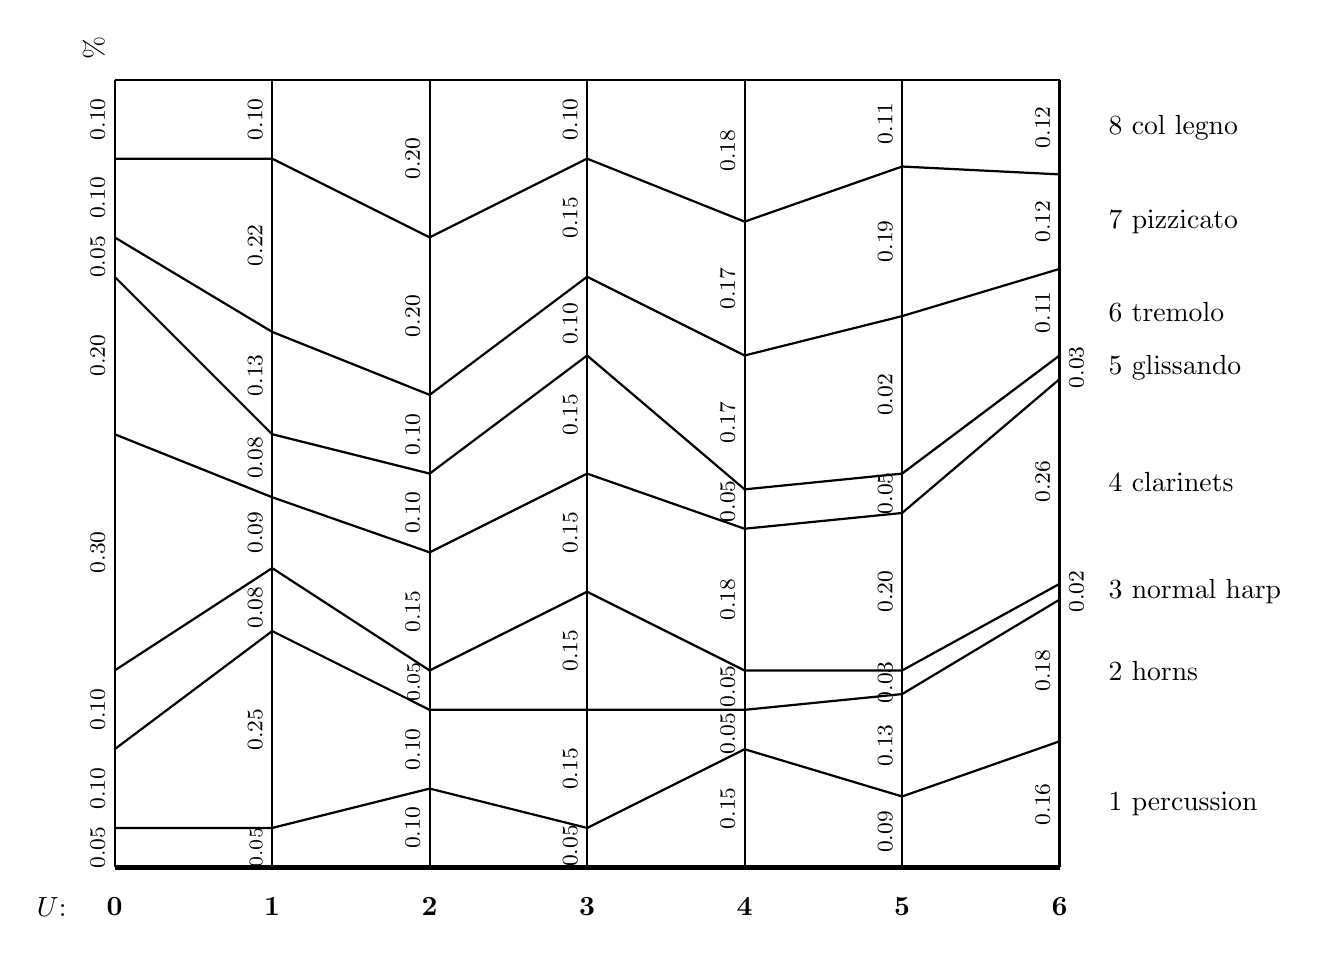
\begin{tikzpicture}[xscale=2, yscale=10]

% vertical lines
\foreach \x in {0,...,6} {
    \draw[thick] (\x, 0) -- (\x, 1);
    \node at (\x, -0.05) {\textbf{\x}};
}

% box lines
\draw[ultra thick] (0,0) -- (6,0);
\draw[thick] (0,1) -- (6,1);

% axis labels
\node at (-0.4, -0.05) {\(U\):};
\node[above, rotate=90] at (0, 1.04) {\%};

% graph lines
\draw[thick] (0,0.05) -- (1,0.05) -- (2,0.10) -- (3,0.05) -- (4,0.15) -- (5,0.09) -- (6,0.16);
\draw[thick] (0,0.15) -- (1,0.30) -- (2,0.20) -- (3,0.20) -- (4,0.20) -- (5,0.22) -- (6,0.34);
\draw[thick] (0,0.25) -- (1,0.38) -- (2,0.25) -- (3,0.35) -- (4,0.25) -- (5,0.25) -- (6,0.36);
\draw[thick] (0,0.55) -- (1,0.47) -- (2,0.40) -- (3,0.50) -- (4,0.43) -- (5,0.45) -- (6,0.62);
\draw[thick] (0,0.75) -- (1,0.55) -- (2,0.50) -- (3,0.65) -- (4,0.48) -- (5,0.50) -- (6,0.65);
\draw[thick] (0,0.80) -- (1,0.68) -- (2,0.60) -- (3,0.75) -- (4,0.65) -- (5,0.70) -- (6,0.76);
\draw[thick] (0,0.90) -- (1,0.90) -- (2,0.80) -- (3,0.90) -- (4,0.82) -- (5,0.89) -- (6,0.88);

% graph labels
\node[above, rotate=90, font=\footnotesize] at (0, 0.025) {0.05};
\node[above, rotate=90, font=\footnotesize] at (0, 0.100) {0.10};
\node[above, rotate=90, font=\footnotesize] at (0, 0.200) {0.10};
\node[above, rotate=90, font=\footnotesize] at (0, 0.400) {0.30};
\node[above, rotate=90, font=\footnotesize] at (0, 0.650) {0.20};
\node[above, rotate=90, font=\footnotesize] at (0, 0.775) {0.05};
\node[above, rotate=90, font=\footnotesize] at (0, 0.850) {0.10};
\node[above, rotate=90, font=\footnotesize] at (0, 0.950) {0.10};

\node[above, rotate=90, font=\scriptsize] at (1, 0.025) {0.05};
\node[above, rotate=90, font=\footnotesize] at (1, 0.175) {0.25};
\node[above, rotate=90, font=\footnotesize] at (1, 0.330) {0.08};
\node[above, rotate=90, font=\footnotesize] at (1, 0.425) {0.09};
\node[above, rotate=90, font=\footnotesize] at (1, 0.520) {0.08};
\node[above, rotate=90, font=\footnotesize] at (1, 0.625) {0.13};
\node[above, rotate=90, font=\footnotesize] at (1, 0.790) {0.22};
\node[above, rotate=90, font=\footnotesize] at (1, 0.950) {0.10};

\node[above, rotate=90, font=\footnotesize] at (2, 0.050) {0.10};
\node[above, rotate=90, font=\footnotesize] at (2, 0.150) {0.10};
\node[above, rotate=90, font=\scriptsize] at (2, 0.235) {0.05};
\node[above, rotate=90, font=\footnotesize] at (2, 0.325) {0.15};
\node[above, rotate=90, font=\footnotesize] at (2, 0.450) {0.10};
\node[above, rotate=90, font=\footnotesize] at (2, 0.550) {0.10};
\node[above, rotate=90, font=\footnotesize] at (2, 0.700) {0.20};
\node[above, rotate=90, font=\footnotesize] at (2, 0.900) {0.20};

\node[above, rotate=90, font=\footnotesize] at (3, 0.027) {0.05};
\node[above, rotate=90, font=\footnotesize] at (3, 0.125) {0.15};
\node[above, rotate=90, font=\footnotesize] at (3, 0.275) {0.15};
\node[above, rotate=90, font=\footnotesize] at (3, 0.425) {0.15};
\node[above, rotate=90, font=\footnotesize] at (3, 0.575) {0.15};
\node[above, rotate=90, font=\footnotesize] at (3, 0.690) {0.10};
\node[above, rotate=90, font=\footnotesize] at (3, 0.825) {0.15};
\node[above, rotate=90, font=\footnotesize] at (3, 0.950) {0.10};

\node[above, rotate=90, font=\footnotesize] at (4, 0.075) {0.15};
\node[above, rotate=90, font=\footnotesize] at (4, 0.170) {0.05};
\node[above, rotate=90, font=\footnotesize] at (4, 0.230) {0.05};
\node[above, rotate=90, font=\footnotesize] at (4, 0.340) {0.18};
\node[above, rotate=90, font=\footnotesize] at (4, 0.465) {0.05};
\node[above, rotate=90, font=\footnotesize] at (4, 0.565) {0.17};
\node[above, rotate=90, font=\footnotesize] at (4, 0.735) {0.17};
\node[above, rotate=90, font=\footnotesize] at (4, 0.910) {0.18};

\node[above, rotate=90, font=\footnotesize] at (5, 0.045) {0.09};
\node[above, rotate=90, font=\footnotesize] at (5, 0.155) {0.13};
\node[above, rotate=90, font=\footnotesize] at (5, 0.235) {0.03};
\node[above, rotate=90, font=\footnotesize] at (5, 0.350) {0.20};
\node[above, rotate=90, font=\footnotesize] at (5, 0.475) {0.05};
\node[above, rotate=90, font=\footnotesize] at (5, 0.600) {0.02};
\node[above, rotate=90, font=\footnotesize] at (5, 0.795) {0.19};
\node[above, rotate=90, font=\footnotesize] at (5, 0.945) {0.11};

\node[above, rotate=90, font=\footnotesize] at (6, 0.080) {0.16};
\node[above, rotate=90, font=\footnotesize] at (6, 0.250) {0.18};
\node[below, rotate=90, font=\footnotesize] at (6, 0.350) {0.02};
\node[above, rotate=90, font=\footnotesize] at (6, 0.490) {0.26};
\node[below, rotate=90, font=\footnotesize] at (6, 0.635) {0.03};
\node[above, rotate=90, font=\footnotesize] at (6, 0.705) {0.11};
\node[above, rotate=90, font=\footnotesize] at (6, 0.820) {0.12};
\node[above, rotate=90, font=\footnotesize] at (6, 0.940) {0.12};

% instrument labels
\node[right] at (6.25, 0.080) {1 percussion};
\node[right] at (6.25, 0.250) {2 horns};
\node[right] at (6.25, 0.350) {3 normal harp};
\node[right] at (6.25, 0.490) {4 clarinets};
\node[right] at (6.25, 0.635) {5 glissando};
\node[right] at (6.25, 0.705) {6 tremolo};
\node[right] at (6.25, 0.820) {7 pizzicato};
\node[right] at (6.25, 0.940) {8 col legno};

\end{tikzpicture}
